%!TEX root = ../thesis.tex
%*******************************************************************************
%*********************************** Energy data appendix *****************************
%*******************************************************************************

\chapter{Cambridge University Estates building energy usage dataset} \label{app:data}

\graphicspath{{Data/Figs/}}


\begin{cbox}[colback=Cerulean!10!white]{}
    \printpublication{langtry2024CambridgeUniversityEstates}

    \noindent{\color{black!50}\rule{\textwidth}{0.4mm}}\vspace{2mm}

    \noindent
    This dataset described in this appendix has been released as the above.\\

    \noindent
    The full dataset can be viewed interactively online at \url{https://eeci.github.io/Cambridge-Estates-Building-Energy-Archive}. Further documentation is available at \url{https://github.com/EECi/Cambridge-Estates-Building-Energy-Archive}.

\end{cbox}

\hfill \\

\noindent
The University of Cambridge has been collecting energy usage data from buildings across its estate for several decades. Thanks to this the University Estates Division has accumulated one of the largest, long-duration building energy usage datasets \citep{kang2023SystematicReviewBuilding}. It is particularly interesting as it covers buildings of widely varying sizes, ages, and usage types, and includes significant changes in energy usage behaviour, for example after buildings have been retrofit.

The scale of this dataset makes it a valuable resource for building energy research. However previously only small sections of the dataset have been used for research \citep{pickering2019DistrictEnergySystem,ward2019DatacentricBottomupModel,ward2021tool,zhuang2023UncertaintybasedOptimalEnergy}. To allow researchers to make use of this data resource for large-scale studies, the dataset has been cleaned, formatted, and made publicly available in an anonymised form. This dataset enabled the studies performed in \Cref{chap:forecasting,chap:districts}, and has already been used by other researchers \citep{choi2025RepresentationVectorBasedTime}.

\newpage
\noindent
The dataset contains historic electricity and gas usage data covering the period 2000 to 2023 from 121 buildings in the Cambridge University Estate of varying use types, such as lecture blocks, offices, laboratories, and museums. Due to issues with the building monitoring, the buildings have sometimes sporadic data availability. However in total, there were 1649 years of electricity data and 600 years of gas data with sufficient data quality which have been made available. Alongside this energy usage data, historic weather data, grid electricity price ,and grid carbon intensity data for Cambridge have been provided. The dataset has also been designed to be compatible with the CityLearn framework \citep{vazquez-canteli2019CityLearnV1OpenAI,vazquez-canteli2020CityLearnStandardizingResearch} to make it easy to simulate building energy system control with real operational data.\\

The energy usage data was collected by building monitoring systems (smart meters) installed in each building. The electricity usage measurements record the total electrical load at a given metering point in the building, which includes lighting, plug loads, and plant equipment  electricity consumption. It is assumed that none of the buildings have heat pumps or AC units, so the electricity usage does not include any contributions from space heating or cooling. The gas usage measurements provide the total gas consumption at the metering points in each building, which is used for both space heating and DHW provision. In the dataset, energy usage data is available at an hourly resolution. The raw data, at a half-hourly resolution, was cleaned by replacing missing values with 0 readings, clipping all values to the range 0 to 10 times the mean of each dataset, and aggregating the data to hourly resolution. Clipping is performed to limit the impact of excessively large observations in the raw data caused by data recording issues in the building monitoring systems.

Hourly weather observation data was collected from the Met Office MIDAS dataset \cite{metoffice2022MIDASOpenUK}. As all buildings in the dataset are closely located, within Cambridge city, the same weather data is used for all buildings. Outdoor dry bulb temperature and relative humidity data are taken from the Bedford measurement station of the MIDAS dataset, the closest location with complete data availability over the period, which provides pre-processed historic weather measurements. Data for direct and diffuse solar irradiance at ground level, and solar generation potential in central Cambridge were collected from the \href{https://www.renewables.ninja/}{renewables.ninja} reanalysis model \citep{pfenninger2016LongtermPatternsEuropean,staffell2016UsingBiascorrectedReanalysis}, which estimates historic solar irradiance values from historic global weather observations. Hourly dynamic electricity pricing tariff data and grid electricity carbon intensity data were collected from Energy Stats UK \citep{energystatsuk2023HistoricalPricingData} and the National Grid ESO Data Portal \citep{nationalgrideso2020HistoricGenerationMix}, respectively. Temporal variables are also provided: month, hour, day of the week, and daylight savings status.\\

\Cref{tab:estates-data-variables} summarises the variables provided in the dataset. Further detail on the data sourcing and processing is available at \url{https://github.com/EECi/Cambridge-Estates-Building-Energy-Archive}. Fig. \ref{fig:estates-data-summary} summarises the data availability across buildings in the dataset.\\

\begin{table}[h]
    \centering
    \renewcommand{\arraystretch}{1.5}
    \begin{tabularx}{\linewidth}{cccY} \toprule \toprule
        Variable & Units & Data availability & \multicolumn{1}{>{\centering\arraybackslash}c}{Data source} \\
        \midrule \midrule
        \multicolumn{4}{>{\centering\arraybackslash}l}{\small\it \quad Building specific variables} \\
        Electrical load & kWh & \multirow{2}{*}{Building dependent} & \multirow{2}{5cm}{\footnotesize Cambridge estates building meters} \\
        Gas load & kWh & & \\
        \midrule
        \multicolumn{4}{>{\centering\arraybackslash}l}{\small\it \quad Location related variables} \\[1ex]
        \makecell{Grid electricity\\price} & £/kWh & 2019 to 2023 & \multirow{1}{5cm}{\footnotesize Energy Stats UK\\\citep{energystatsuk2023HistoricalPricingData}} \\
        \arrayrulecolor{black!50}\midrule
        \makecell{Grid electricity\\carbon intensity} & kgCO$_2$/kWh & 2009 to 2023 & \multirow{1}{5cm}{\footnotesize National Grid ESO data portal\\\citep{nationalgrideso2020HistoricGenerationMix}} \\
        \arrayrulecolor{black!50}\midrule
        \makecell{Solar generation\\potential} & W/kWp & \multirow{3}{*}{All} & \multirow{3}{5cm}{\footnotesize \href{https://www.renewables.ninja/}{renewables.ninja} reanalysis model\\\citep{pfenninger2016LongtermPatternsEuropean}\\\citep{staffell2016UsingBiascorrectedReanalysis}} \\
        \makecell{Direct solar\\irradiance} & W/m$^2$ & & \\
        \makecell{Diffuse solar\\irradiance} & W/m$^2$ & & \\
        \arrayrulecolor{black!50}\midrule
        Outdoor temperature & \textdegree{}C & \multirow{2}{*}{2000 to 2022} & \multirow{2}{5cm}{\footnotesize Met Office MIDAS dataset\\\citep{metoffice2022MIDASOpenUK}} \\
        Relative humidity & \% & & \\
        \arrayrulecolor{black!50}\midrule
        Time information & -- & All & -- \\
        \arrayrulecolor{black}\bottomrule \bottomrule
    \end{tabularx}
    \smallskip
    \caption{Summary of variables available in dataset.} \label{tab:estates-data-variables}
\end{table}

\begin{figure}
    \centering
    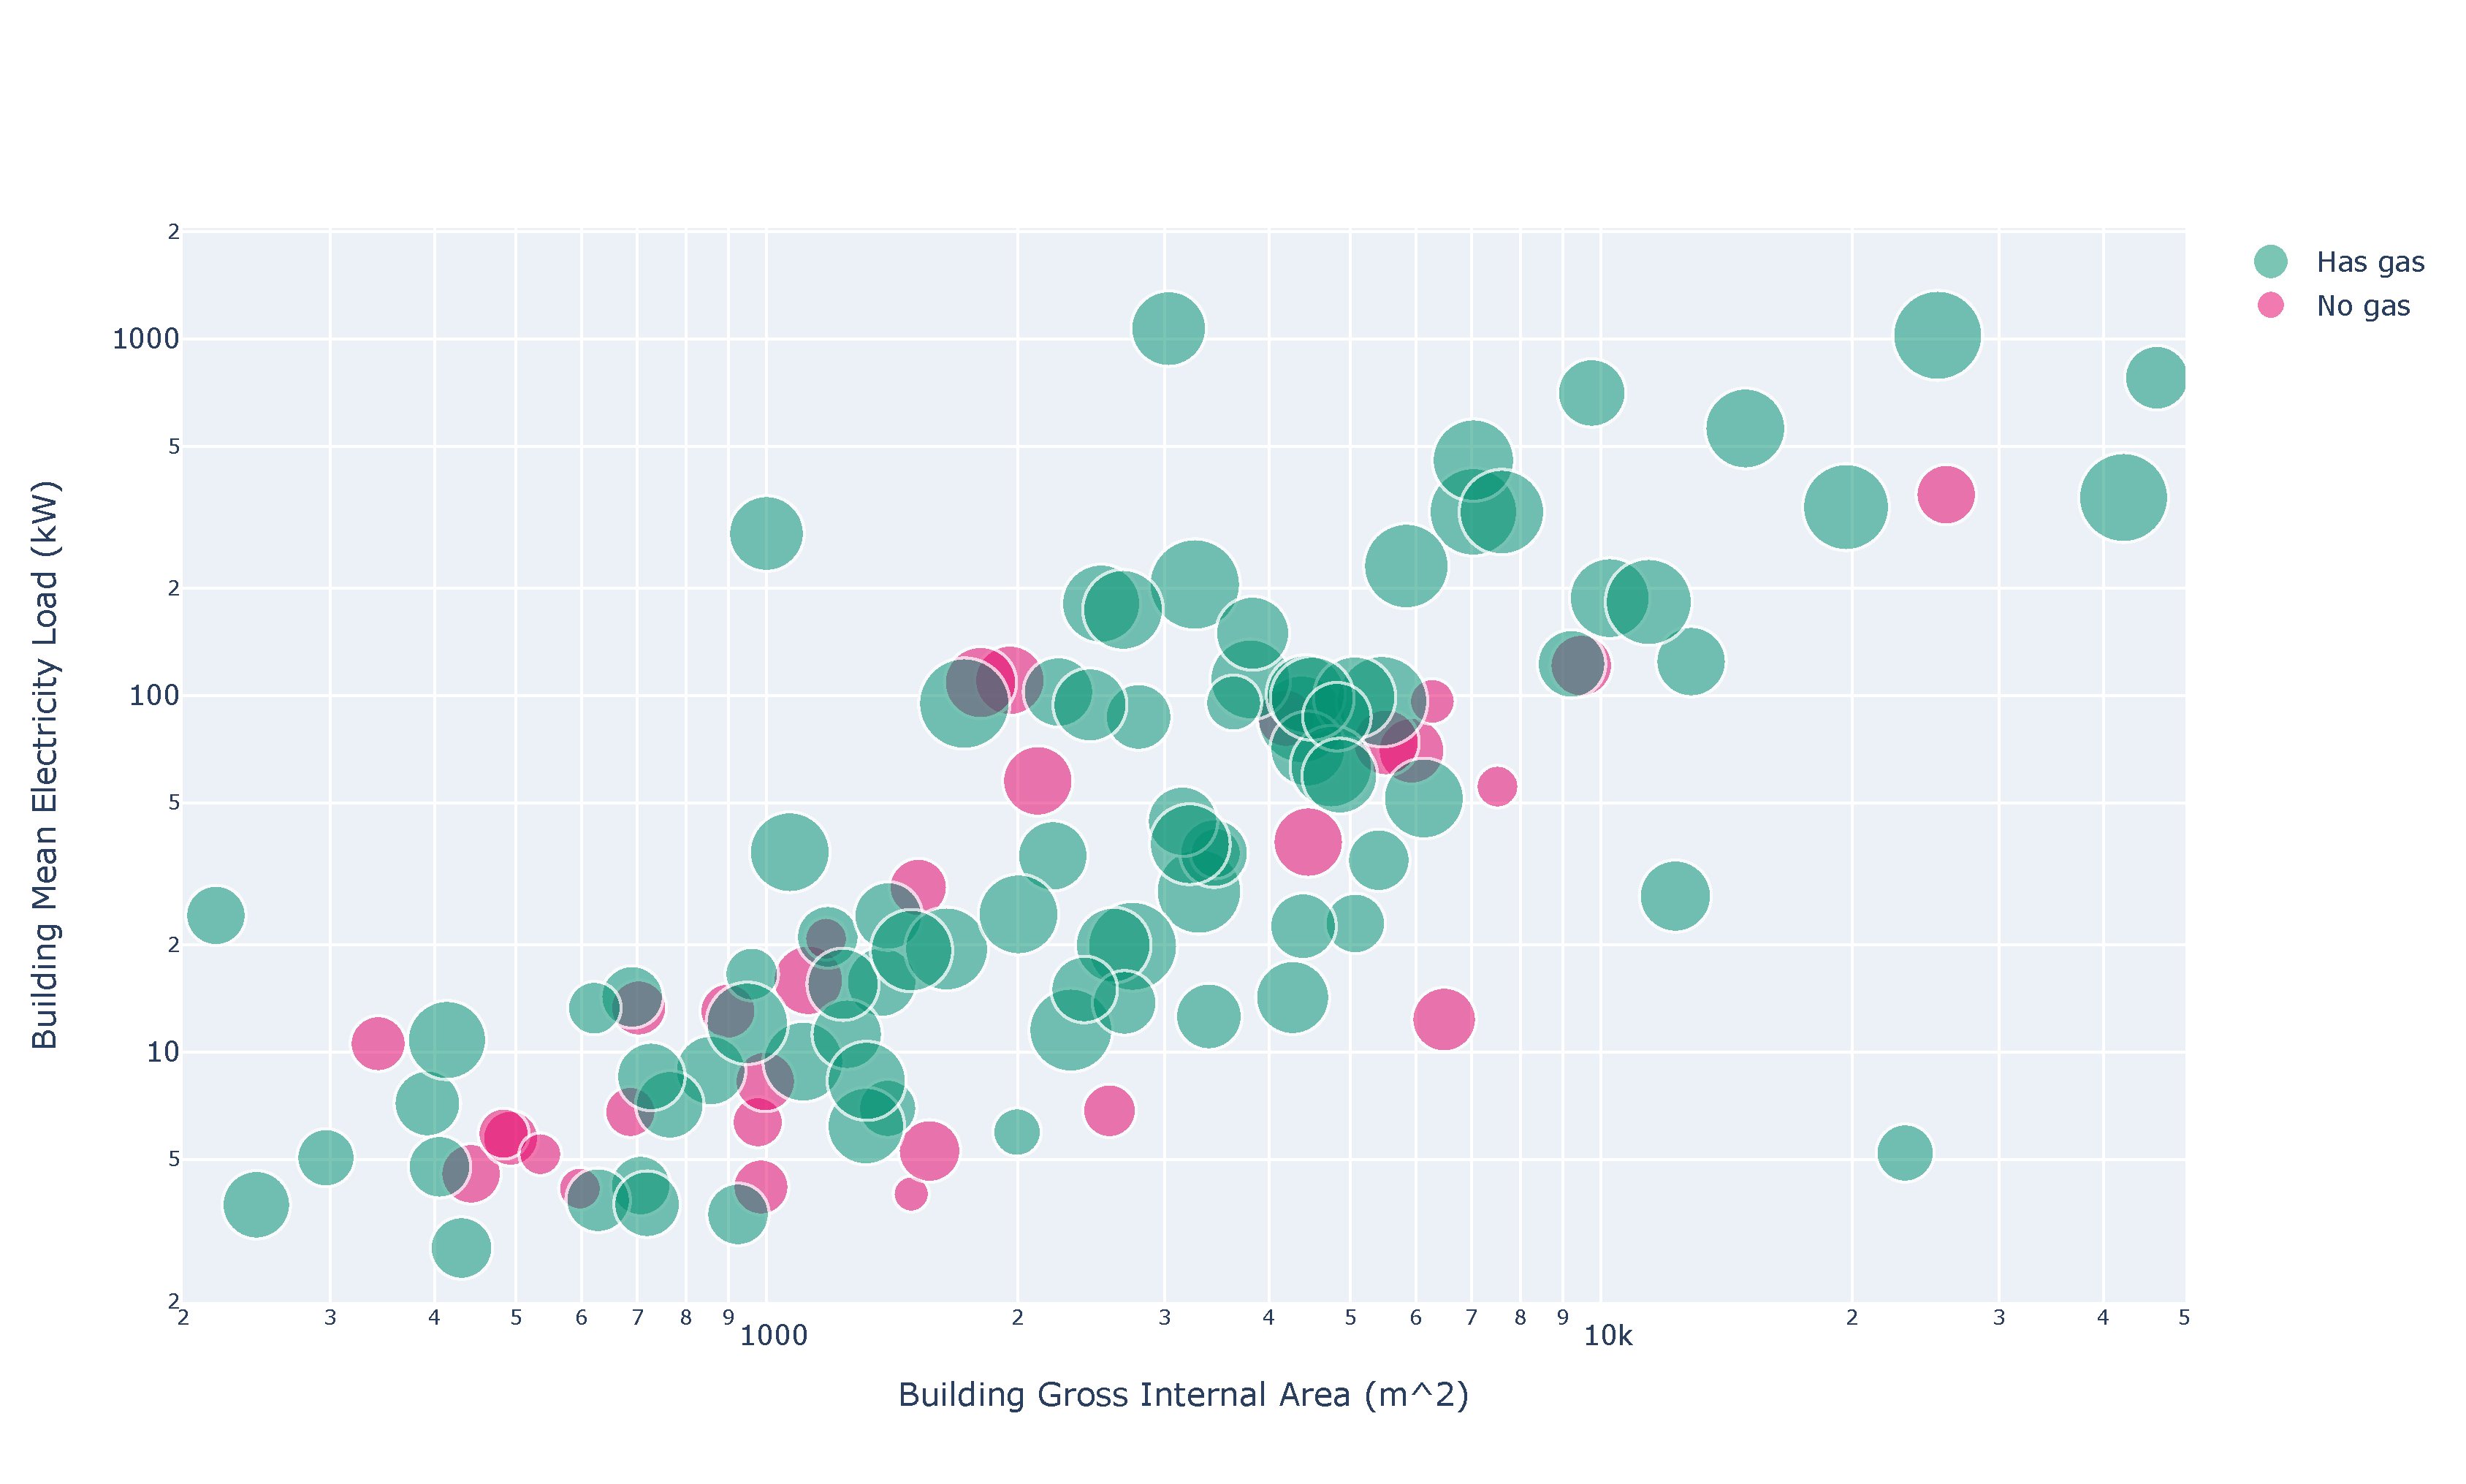
\includegraphics[width=\linewidth]{dataset_summary.pdf}
    \vspace*{-1cm}
    \caption{Summary of data availability across buildings in dataset.} \label{fig:estates-data-summary}
    \vspace{0.2cm}
    \footnotesize{\textit{Interactive version of plot available online} \href{https://eeci.github.io/Cambridge-Estates-Building-Energy-Archive/building_data_summary.html}{\textbf{here}}.}
\end{figure}